\chapter{Approche et Implémentation}

\section*{Introduction}
Dans ce chapitre nous présenterons premièrement les données qui ont été utilisés
pour entrainer notre modèle. Ensuite, nous présenterons les résultats obtenus à
la suite de l'utilisation des algorithmes sur nos données. Enfin nous 
présenterons les perspectives envisagées.
Quelle approche est la mieux adaptée à nos besoins? Choisir un algorithme 
d’apprentissage supervisé ou non supervisé dépend habituellement de 
facteurs liés à la structure et au volume de nos données, et le cas 
d’utilisation auquel nous voulons l’appliquer.


\section{Approche}

L'objectif de notre travail est de mettre en place un système permettant 
d'analyser ou de réaliser la mise en conformité d'une opération à l'étranger et
de tous les acteurs intervenants dans cette opération. Cette analyse se base
sur le dossier que le client a fourni au guichet des opérations 
internationales.

L'analyse conformité regroupe plusieurs activités que nous ne considèrerons pas
toutes dans un premier temps. En effet, dans le but d'avoir un modèle
beaucoup plus efficace, nous nous focaliserons tout d'abord sur :
\begin{itemize}
  \item La détection des transactions suspectes
  \item l'allègement des procédures KYC
\end{itemize}
Pour atteindre les objectifs que nous nous sommes fixés, nous considérons un
dossier d'opération comme l'ensemble des informations contenues sur chaque
élément du dossier. Un dossier d'opération est donc l'ensemble des
caractéristiques entrant en compte dans la détection d'une transaction suspecte
et des informations d'identification de tous les intervenants à l'opération.
Ces informations sont relevées directement sur le dossier physique transmis 
par le client.

La détection d'anomalies dans notre cas n'a pas fourni de résultats 
satisfaisants. En effet, elles éliminent une énorme partie des données d'entrées, qui
ne représentent pas forcément des anomalies. Nous avons donc chercher d'autres
méthodes pour la résolution de notre problème.
Pour cela, la méthode adoptée pour la mise en place du système devra respecter les
exigences bancaires à savoir que la mise à jour du sytème doit être 
possible et la décision prise expliquable et le système sécurisé.
En somme, le modèle ne devra pas fonctionner comme une boîte noire.

Parmi les principaux algorithmes de classification connus, ceux ne
fonctionnant pas comme une boite noire sont l'algorithme des plus proches
voisins(K-NN) et celui des arbres de décisions(Décision Tree). Les arbres de
décisions offrent l'avantage de pouvoir générer des règles de décisions pour
toutes les différentes classifications qui sont réalisées. C'est la méthode qui
sera utilisée pour réaliser notre modèle d'apprentissage.

Nous posons comme hypothèse de départ que tous les dossiers sont complets et 
conformes à la règlementation de change avant de passer par le modèle
d'aprentissage. Cette hypothèse nous permet de nous focaliser sur les autres
aspects de la conformité qui ont été cités précédemment.

\section{Réalisation}

\subsection{Le jeu de données}

\subsubsection{Acquisition des données}

Les moyens à mettre en oeuvre au sein des banques pour appliquer de manière
opérationnelle les recommandations du GAFI et se conformer ainsi aux
réglementations en vigueur (ordonnance 2009-104, code monétaire et financier)
implique un processus approfondi de connaissance du client et le contrôle et
la surveillance des transactions.

Les éléments présents sur un dossier et permettant de connaitre un client
intervenant dans une opération(client émetteur ou destinataire de l'opération)
sont:
\begin{itemize}
  \item le type de personne (personne physique ou morale)
  \item l'identité de la personne
  \item le pays de résidence de la personne
  \item la banque de la personne
  \item le pays dans lequel cette banque se trouve
\end{itemize}
Tous les éléments cités ci-dessus doivent être contrôlés sur les listes
officielles de vérification de sanctions et d'embargo. Le résultat de chacun
de ces contrôles est indispensable pour effectuer l'analyse d'une opération.

Les informations présentes sur un dossier et permettant de contrôler ou
surveiller une transaction en cours sont:
\begin{itemize}
  \item L'activité de l'émetteur de l'opération
  \item l'activité du bénéficiaire de l'opération
  \item l'objet de l'opération(salaire, achat d'une voiture, de frais
    médicaux\ldots)
  \item le type de l'opération(transfert émis, transfert recu,  credoc,
    remdoc\ldots)
  \item le montant de l'opération
  \item la dévise de l'opération
\end{itemize}

En somme, Pour inférer correctement sur de nouvelles données, les jeu de
données qui seront utilisés pendant la phase d'apprentissage auront les
caractéristiques suivantes :

\begin{itemize}
  \item le type de personne du donneur (personne physique ou morale)
 \item l'identité de l'émetteur et le résultat de son contrôle sur les
   listes de sanctions
 \item le pays de résidence de l'émetteur et sa notation
 \item la banque de l'émetteur et le résultat de son contrôle sur les
   listes de sanctions
 \item le pays dans lequel cette banque se trouve et sa notation
 \item le type de personne du bénéficiaire (personne physique ou morale)
 \item l'identité du bénéficiaire et le résultat de son contrôle sur les
   listes de sanctions
 \item le pays de résidence du bénéficiare et sa notation
 \item la banque du bénéficiaire et le résultat de son contrôle sur les
   listes de sanctions
 \item le pays dans lequel cette banque se trouve et sa notation
 \item l'activité de l'émetteur de l'opération
 \item l'activité du bénéficiaire de l'opération
 \item l'objet de l'opération(salaire, achat d'une voiture, de frais
    médicaux \ldots
 \item le type de l'opération(transfert émis, transfert recu,  credoc,
    remdoc...)
 \item le montant de l'opération
 \item la dévise de l'opération
\end{itemize}

Comme nous ne disposions pas de toutes ces informations sur des fichiers, nous
avons, en collaboration avec les colaborateurs du service des opérations
internationales et ceux de la Direction Conformité, constitué un jeu de données
afin de réaliser notre apprentissage.


\subsection{Prétraitrement des données}

Les caractéristiques recencées ci-dessus nous permettent de juger de la 
conformité d'un dossier de transferts. Certaines caractéristiques sont très
distinctives et pourraient entrainées un sur-apprentissage de notre modèle.
Il s'agit par exemple de 
\begin{itemize}
  \item l'identité de l'émetteur de l'opération
  \item le pays de résidence de l'émetteur 
  \item la banque de la l'émetteur
  \item le pays dans lequel cette banque se trouve
  \item l'identité du bénéficiaire de l'opération
  \item le pays de résidence du bénéficiaire de l'ordre
  \item la banque du bénéficiaire
  \item le pays dans lequel cette banque se trouve
  \item la dévise de l'opération
\end{itemize}

Dans le tableau \ref{tab:tab3}, nous présentons l'ensemble des caractéristiques de
notre jeu de données. Celles qui sont en italiques représentent les 
caractéristiques d'entrée de notre algorithmes de machine learning.


\begin{table}

  \begin{center}
    \begin{scriptsize}
      \renewcommand{\arraystretch}{2}
      \begin{tabular}{|c|l|l|}
        \hline
        \rowcolor[gray]{.7}
        \bf \rule[-0.4cm]{0mm}{1cm} Section & \bf Caractéristiques & \bf Exemples\\
        \hline
        \multirow{7}{*}{\bf Emetteur de l'ordre} & \textit{Type de personne} & Personne 
        physique 
        \tabularnewline
        & Identité & XXXXXX XXXXXX \tabularnewline 
        & \textit{Résultat du contrôle de l'émetteur} & Aucune sanction  \tabularnewline
        & Pays de résidence & Burkina Faso \tabularnewline
        & \textit{Notation du pays de résidence} & LOW \tabularnewline
        & Banque de l’émetteur & SGBF \tabularnewline
        & Pays de la banque & Burkina Faso \tabularnewline
        & \textit{Notation Pays de la banque} & LOW \tabularnewline
        & \textit{Résultat du contrôle sur la banque} & Aucune sanction  \tabularnewline
        & \textit{Activité de l'emetteur} & Activités extractives \tabularnewline 
        \hline

        \multirow{7}{*}{\bf Bénéficiaire de l'ordre} & \textit{Type de personne} & Personne
        morale 
        \tabularnewline
        & Identité & ZZZZZZZZZZ \tabularnewline
        & \textit{Résultat du contrôle sur la personne} & Aucune sanction  \tabularnewline
        & Pays de résidence & France \tabularnewline 
        & \textit{Notation du pays de résidence} & LOW \tabularnewline
        & Banque de l’émetteur & BNP Paribas \tabularnewline
        & Pays de la banque & France \tabularnewline 
        & \textit{Notation Pays de la banque} & LOW \tabularnewline
        & \textit{Résultat du contrôle de la banque} & Aucune sanction  \tabularnewline
        & \textit{Activité du bénéficiaire} & Hébergement et hôtellerie  \tabularnewline 
        \hline
        \multirow{5}{*}{\bf Opération} & Type  & Règlement de facture \tabularnewline
        & \textit{Objet}  & Frais d'hébergement \tabularnewline
        & \textit{Montant}& 25000 \tabularnewline
        & Devise & Euros \tabularnewline

        \hline
      \end{tabular}
    \end{scriptsize}
    \caption{Exemple de dossier d'opération conforme \label{tab:tab3}}
  \end{center}
\end{table}


Le jeu de données final qui a servi pour l'apprentissage et les tests  est constitué de
six cent (600) dossiers d'opérations.


Pour des questions pratiques, nous avons constitué un dictionnaire des
différents secteurs d'activités ainsi que des objets de transactions.
Un échantillon du dictionnaire est présenté au tableau \ref{tab:codage}.
\begin{table}
 \begin{center}
    \begin{scriptsize}
      \renewcommand{\arraystretch}{2}
      \begin{tabular}{|m{5cm}|m{2cm}||m{5cm}|m{2cm}|}
        \hline
        \rowcolor[gray]{.7}
        \bf \rule[-0.4cm]{0mm}{1cm} Libellé secteur d'activité & \bf Code &
        \bf Libelle du secteur d'activité & \bf Code \\
        \hline

      Activités extractives & 0 &  Activités financières & 15 \\
      Agriculture et chasse & 1 & Hôtels et restauration & 3 \\
      Industrie & 4 & Activites de ménages & 5 \\
      Activités des organisations extraterritoriales & 6 & Activités financières & 7 \\
      Commerce gros & 8 & Santé et action sociale & 8 \\
      Administration publique & 9 & Commerce détail\\
      Transport & 10 & Education & 11 \\
      Développements logiciels & 12 & Maintenance de materiels informatiques & 13\\
      Fabrication Produits pharmaceutiques & 16 & Construction & 17 \\
      Fabrication de meubles & 18 & Activités associatives & 19 \\
      Commerce détail & 20 & Fabrication chaussures & 21 \\
      Télécommunications & 22 & Activités Juridiques & 23 \\
      Fabrications produits alimentaires & 24 & Service immobilier & 25 \\
      Fabrication de boissons & 26 & Pêche et pisciculture & 27 \\
        \hline
      \end{tabular}
      \end{scriptsize}
      \caption{Codage de quelques secteurs d'activités\label{tab:codage}}
  \end{center}
\end{table}

    \subsection{Validation croisée et stratification des données}

    \subsubsection{Validation croisée}
      Pour nous assurer que notre modèle ne souffre pas de sur-apprentissage, et
      qu’il saura faire des prédictions sur de nouvelles données, nous avons
      implémenté la validation croisée sur notre modèle de Decisions Tree. La 
      validation croisée va nous permettre d’utiliser l'intégralité de notre jeu
      de données pour l’entraînement et pour la validation.

      Pratiquement, il s'agit de dcouper le jeu de données en $k$ parties(folds
      en anglais) à peu près égales. Tour à tour, chacune des $k$ parties est
      utilisée comme jeu de test. Le reste(autrement dit l'union de $k-1$ autres
      parties) est utilisé pour l'entrainement.
      La validation croisée permet d'éviter un biais potentiel lié au fait de
      faire une évaluation unique.

      \subsubsection{Stratification}


    Le jeu de données dont nous disposons n'est pas équilibré i-e le nombre de
    dossiers non conformes est plus élevé que celui des dossiers conformes. La
    stratification permet d'éviter que les données d'entrainements ne
    contiennent que des exemples positifs et les données de test que des
    exemples négatifs, ce qui affecte négativement les performances du modèle.


\subsection{Les outils}
Nous allons présenter quelques outils qui nous ont permis de mettre en place
le modèle et la plateforme que nous avons proposée. Chaque étape dans la
mise en place d'un modèle de machinelearning possède des outils spécifiques
associés.
\subsubsection{Le langage python}
\begin{wrapfigure}[5]{l}{3.5cm}
  \vspace{-7mm}
  
\includegraphics[width=3cm]{images/python.png}
\end{wrapfigure}

Python a été utilisé pour les codes d'implémentation de notre
modèles. Il s'agit d'un langage de programmation, dont la première version 
est sortie en 1991. Ce langage a été baptisé ainsi en hommage à la troupe de
comiques les \og Monty Python \og.
Python est un langage puissant riche en possibilités et dont les fonctionnalités
peuvent être étendues grâce à de nombreuses bibliothèques. Ainsi, nous avons
utilisé de nombreuses bibliothques python afin de mettre en oeuvre notre modèle.

\begin{description}
  \item[\textbf{Pandas et numpy: }] Pour le nettoyage et l'exploration de nos
      données, les librairies \textbf{Pandas} et \textbf{Numpy} ont été utilisées.
      Pandas permet de créer des tableaux ou dataframes à partir des données
      brutes.
    \item[\textbf{Scikit-learn: }] Tensorflow et Scikit-learn sont les librairies
        les plus utilisées pour la modélisation. Pour notre modèle, le choix a
        été fait d'utiliser \textbf{Scitit-learn}. Ce choix se justifie par le
        fait qu'il implémentedirectement et de manière didactique les différents
        algorithmes d'apprentissage automatique.
    \end{description}
\subsubsection{Le langage Javascript} 

\begin{wrapfigure}[5]{r}{3.5cm}
  \vspace{-7mm}
  
\includegraphics[width=3cm]{images/javascript.png}
\end{wrapfigure}
JavaScript est un langage de programmation de scripts principalement employé
dans les pages web interactives mais aussi pour les serveurs avec 
l'utilisation (par exemple) de Node.js. A travers le framework angular qui est
un framework Javascript, il nous a permis de réaliser une interface
conviviale qui permettrait l'utilisation de notre modèle.

\subsubsection{Flask}
\begin{wrapfigure}[5]{l}{3.5cm}
  \vspace{-7mm}
  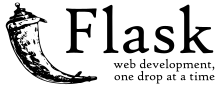
\includegraphics[width=3cm]{images/flask.png}
\end{wrapfigure}

Flask est un framework open-source de développement web en Python. Son but 
principal est d'être léger, afin de garder la souplesse de la programmation
Python, associé à un système de templates. Ils nous a permis de mettre à 
disposition de notre client javascript le modèle python qui a été implémenté.

\subsubsection{Jupyter Notebook}
\begin{wrapfigure}[5]{r}{3.5cm}
  \vspace{-7mm}
  
\includegraphics[width=3cm]{images/jupyter.png}
\end{wrapfigure}

Le Jupyter Notebook est une application web open-source qui vous permet de 
créer et de partager des documents contenant du code interprété en direct, 
des équations, des visualisations et du texte narratif. Les utilisations 
comprennent : le nettoyage et la transformation de données, la simulation 
numérique, la modélisation statistique, la visualisation de données, 
l'apprentissage machine, et bien plus encore. Il est l'un des outils  
du projet Jupyter.

\subsubsection{Visual studio code}

Visual studio code est un éditeur de code édité par microsoft. Il est utilisé
par les développeurs pour la progammer dans de nombreux langages de
programmation. 


 \section{Résultats}
Rappelons que l'objectif de notre étude est mettre en place un système
permettant de classifier une opération(dossier de transfert) à l'étranger selon
la conformité. Un tel système se compose de deux parties. La première partie est
un modèle de machine learning réalisé grâce aux algorithmes de décision Tree. La
seconde est une application permettant d'envoyer à partir d'un formulaire les
éléments du dossier au modèles de Machine Learning.

Nous présenterons tout d'abord les résultats du modèle. Par la suite, nous
montrerons l'application qui permettra une utilisation du modèle.

  \subsection{Résultats du modèle}
  Le modèle classe les dossiers opérations en deux groupes: un groupe
  représentant l'étiquette dossier conforme, l'autre représentant l'étiquette
  dossier non-conforme. Nous étiquettons un dossier conforme \textit{1} et un
  dossier non-conforme \textit{0}
  Les mesures détaillés des test par catégorie sont représentés sur les figures suivantes.

     \begin{figure}[h!]
        \begin{center}
          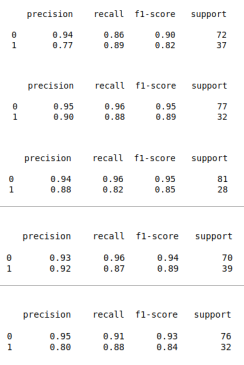
\includegraphics{images/all222.png}
          \caption{Résultat du test. \label{fig:result}}
        \end{center}
      \end{figure}

  Notre test nous révèle un f1-score toujours élevé pour les dossier étiquetés 0
c'est-à-dire pour les dossiers non-conformes. La moyenne de prédiction juste
globale est de $61.31\%$.

Les arbres de décisions étant considérés comme des classifieurs faibles, nous
avons appliqué sur nos données un modèle de forêts aléatoire afin de comparer
ces résultats avec ceux issus d'un arbre de décision simple.

Les résultats obtenues pour un modèle de forêt aléatoire sont présentés dans la 
figure ci-dessous. \ref{fig:randomresult}
 \begin{figure}[h!]
  \begin{center}
    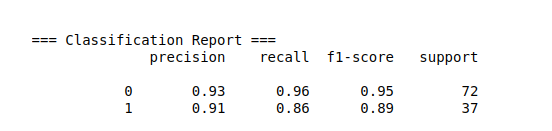
\includegraphics[width=14cm]{images/randomresult.png}
    \caption{Résultat de l'entrainement avec Random
    Forest\label{fig:randomresult}}
  \end{center}
\end{figure}

Ce second test révèle toujours un f1-score toujours  élévé pour les dossiers
non-conformes. La moyenne de prédiction juste est cette fois-ci de 83\%. 

\subsection{Implémentation de la plateforme web}

Pour pouvoir être utilisé par les collaborateurs de la SGBF, le modèle d'analyse
des dossiers qui a été implémenté devra être utilisable à travers une interface
utilisateur conviviale. 
Cette interface en plus d'envoyer des données au modèle, devrait permettre de
contrôler l'intégrité et la fiabilité des acteurs de l'opération. Les
fonctionnalités attendus sont:
\begin{itemize}
  \item Permettre l'enregistrement de toutes les informations concernant une
    nouvelle opération dans une base de données.
  \item Faciliter la vérification sur les différentes listes officielles de
    sanctions et d'embargo.
  \item Permettre une traçabilité des opérations de l'entrée en relation
    jusqu'à l'exécution de l'opération
\end{itemize}

Ainsi, la plateforme qui a été mise en oeuvre permet aux collaborateurs du services 
OPI de renseigner les informations présent dans le dossier et permettant de 
juger de la conformité d'une opération.

A la réception d'un dossier, le collaborateur renseigne les informations sur la
transation sur l'interface présentée sur la figure \ref{fig:transaction}. Les
informations sur l'émetteur de l'ordre sont saisies sur l'écran de la figure \ref{fig:emetteur},
celle sur le bénéficiaire sur l'écran présenté à la figure \ref{fig:beneficiaire}.

A l'enregistrement, les informations sont transmises au modèle pour analyse. Le résultat
de l'analyse est affiché sur l'écran de la figure \ref{fig:analyse}. On retrouve
sur cet écran, le sommaire des informations sur l'émetteur, sur le bénéficiaire
et sur l'opération elle-même.
%Les informations transmises sont codés comme présenté dans la figure ....


\begin{figure}[h!]
  \begin{center}
    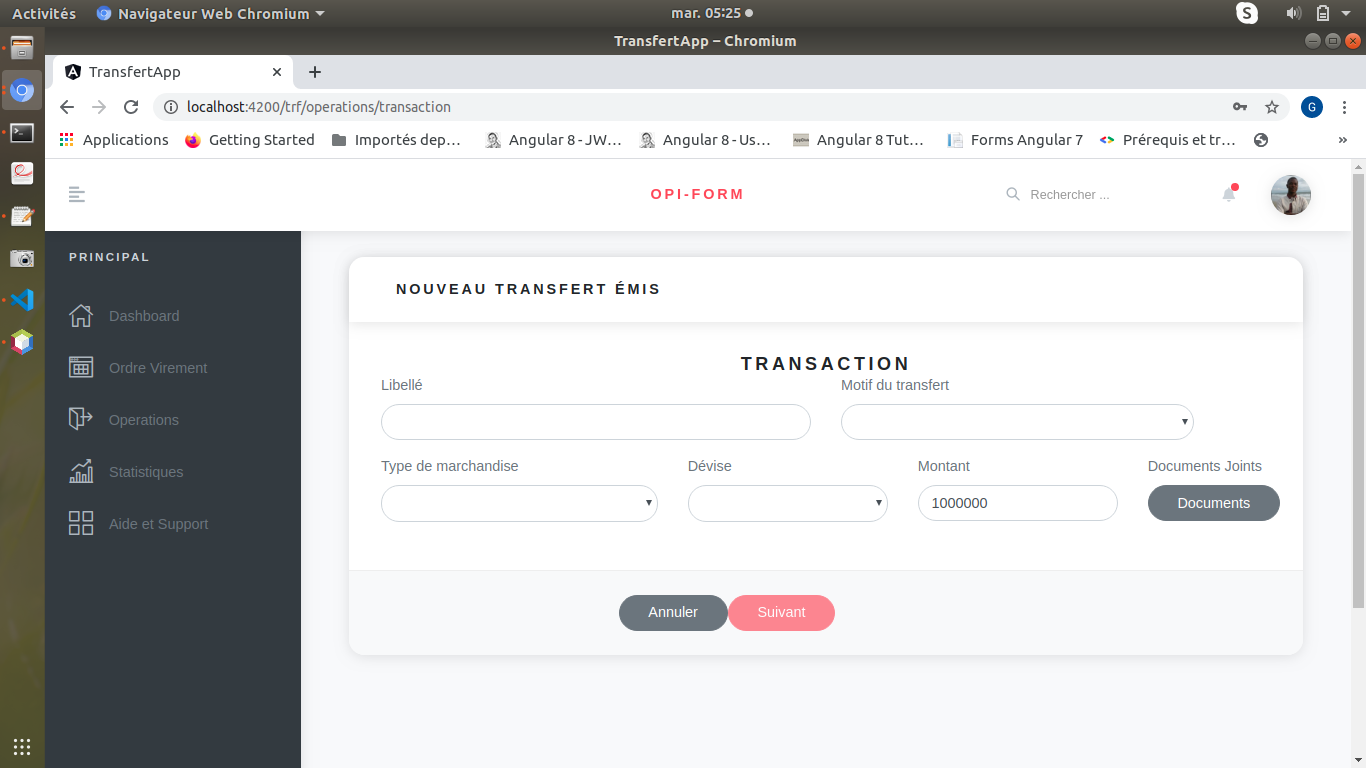
\includegraphics[width=14cm]{images/transaction.png}
    \caption{Ecran de renseignement des informations sur la transaction.\label{fig:transaction}}
  \end{center}
\end{figure}


\begin{figure}[h!]
  \begin{center}
    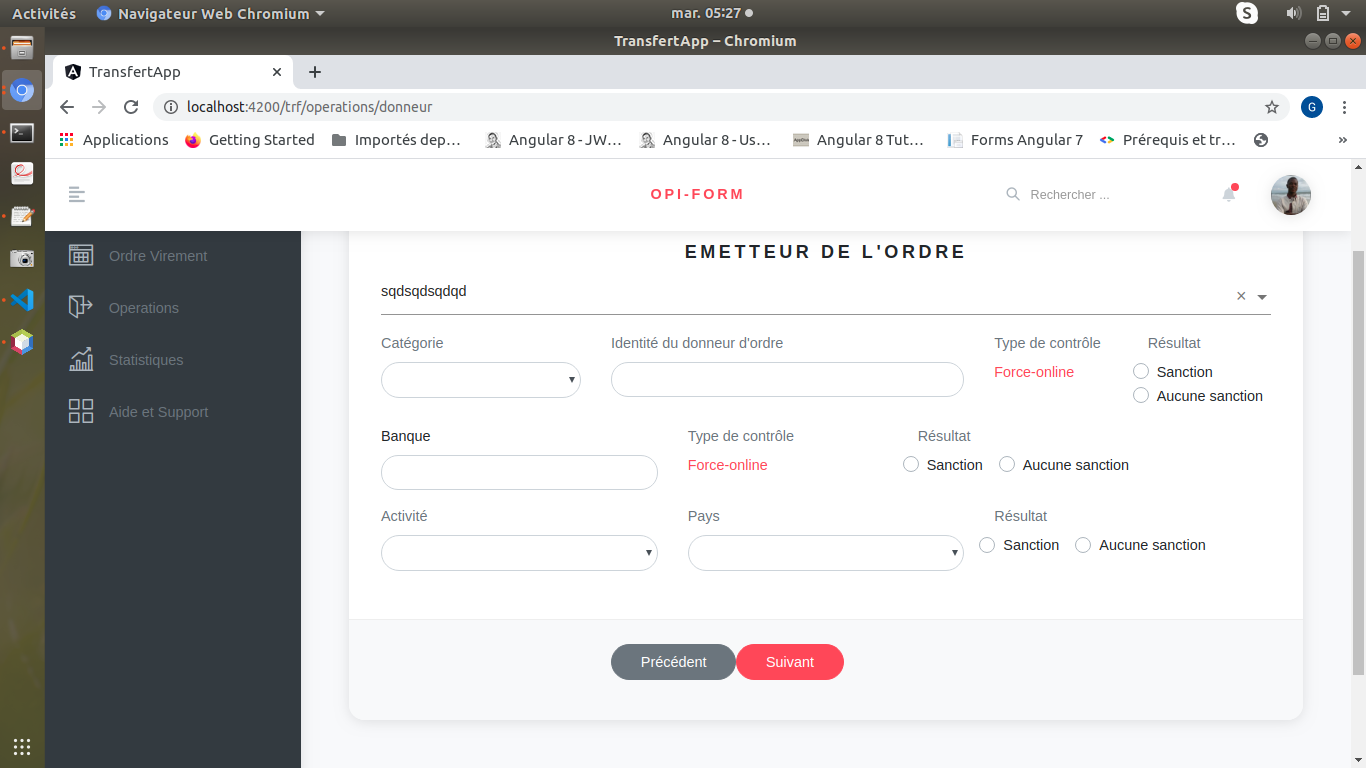
\includegraphics[width=14cm]{images/emetteur.png}
    \caption{Ecran de renseignement des informations sur l'émetteur de l'ordre.\label{fig:emetteur}}
  \end{center}
\end{figure}

\begin{figure}[h!]
  \begin{center}
    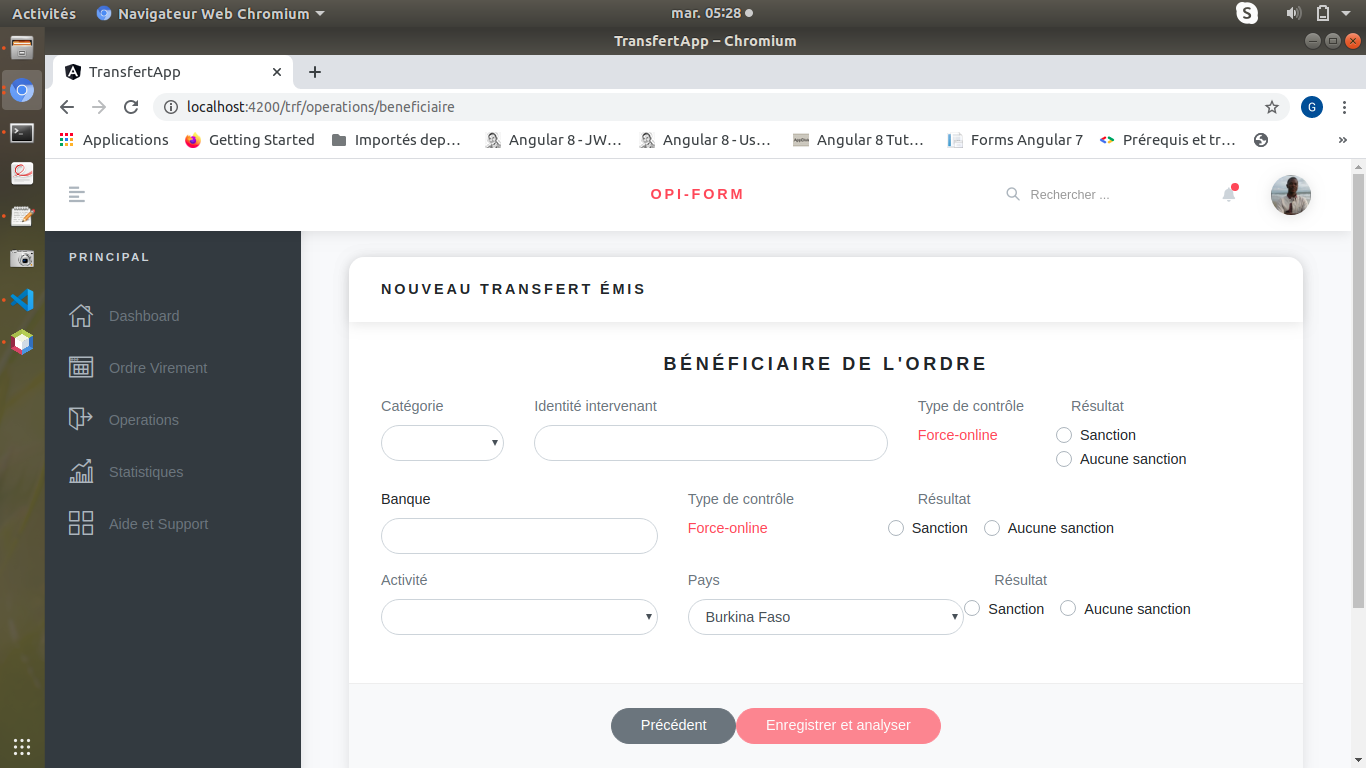
\includegraphics[width=14cm]{images/beneficiaire.png}
    \caption{Ecran de renseignement des informations sur le bénéficiaire de l'ordre.\label{fig:beneficiaire}}
  \end{center}
\end{figure}

\begin{figure}[h!]
  \begin{center}
    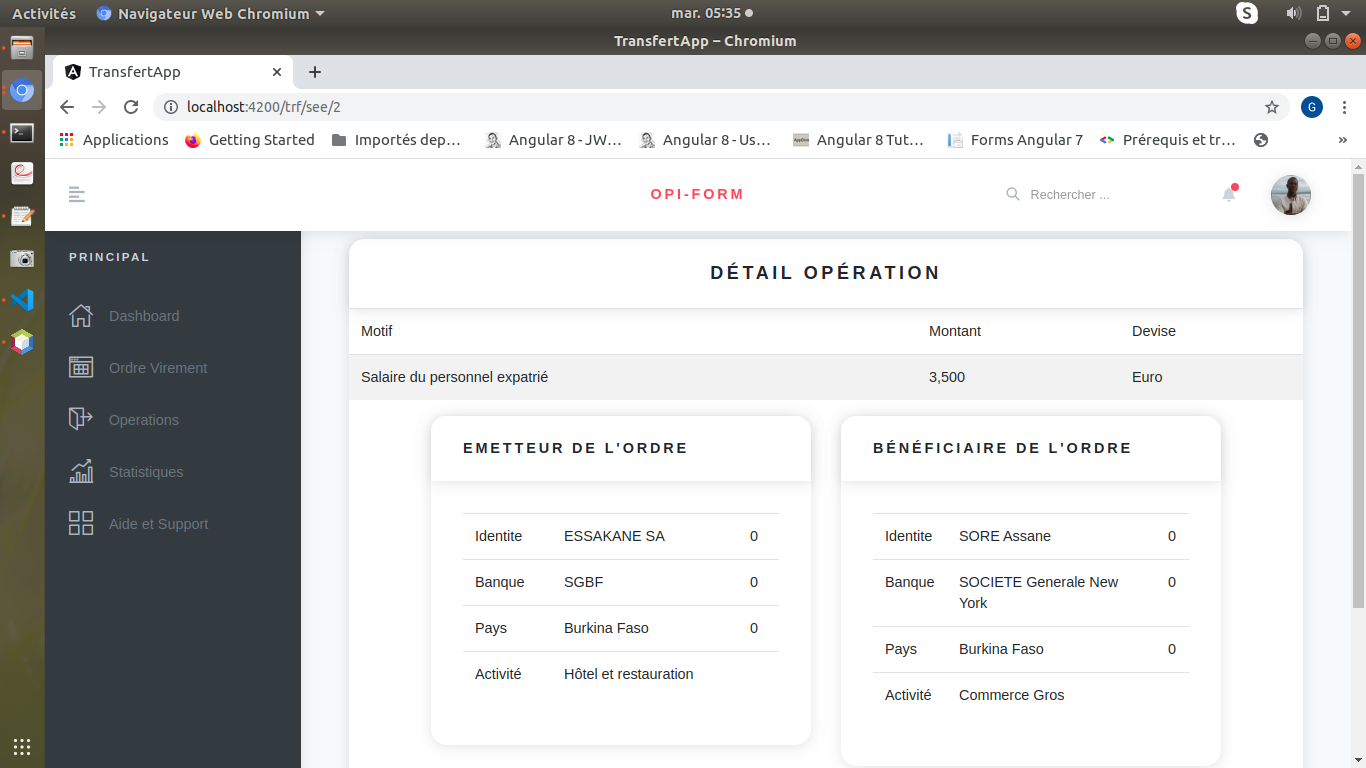
\includegraphics[width=13cm]{images/analyse.png}
    \caption{Ecran de présentation des détails et du résultat de l'analyse .\label{fig:analyse}}
  \end{center}
\end{figure}

   \section{Interprétation des résultats du modèle de machine learning}

  \subsection{Limites et difficultées}

  Sans passer par mille chemins, notre stage était miné de difficultés 
  d’ordre organisationnelles au sein de la banque et des difficultés 
  techniques rencontrées tous les jours.

  Les difficultés organisationnelles sont dues à l'acquisition et à la
  manipulation des données dont nous avions besoin pour l'implémentation de
  notre modèle. En IA, il est une barrière qui demeure impossible à franchir.
  \og Pas de datas, pas d'IA \fg. La principale difficulté a été l'obtention
  des données pour notre modèle. Les  modèles de machine learning se 
  construisent à partir d'exemples d'apprentissage basés sur l'expérience 
  passée. Disposer d'exemples est donc indispensable. Dans le même temps, ces
  exemples doivent être présents et suffisamment en grand nombre pour parvenir à
  une IA généralisable et applicable sur le terrain.

 Cette étape a été la plus difficile car elle a mis à contribution de nombreux 
 collaborateurs de plusieurs services différents(DCO, OPE). Cela nous a permis
 d'obtenir un jeu de données pour l'apprentissage.

  Les difficultés techniques sont liées au choix des différents outils
  d'implémentations du modèle, les pare-feux de la SGBF n'autorisant pas 
  l'installation de certaines applications sur les machines du réseau. Pour les
  outils dont l'installation était impossible, il fallait donc trouver d'autres
  permettant de faire la même tâche beaucoup plus difficilement.

    \subsection{Analyse des résultats}
 La matrice de confusion permet de résumer et visualiser les résultats d'un
 problème de classification. Des mesures permettent d'analyser la matrice de 
 confusion. Ce sont
 \begin{description}
   \item{La précision}: Elle permet de calculer le taux de classification juste.
     C'est la proportion des prédictions correctes parmi les points que l'on a
     prédit.
     $$
     Precision = \frac{VP}{VP + FN}
     $$
   \item{Le rappel ou sensibilité: } En anglais \textit{recall}, il donne la proportion des
     exemples bien étiquetés.
     $$
     Rappel = \frac{VP}{VP + FP}
     $$
   \item{L'exactitude: } En anglais \textit{accuracy}, il évalue le taux de
     bonnes réponses.
     $$
     Accuracy = \frac{VP + VN} {Vp + FP + VN + FN}
     $$
   \item{F1-score} Il s'agit de la moyenne harmonique de la précision et du
     recall. Il reflète les différents aspects du modèle.
     $$
     F1 = 2 * \frac{Precision * Rappel}{Precision + Rappel}
     $$
 \end{description}
   
 Les résultats obtenus après évaluation de notre modèle de classiication font
 ressortir quelques éléments.
 Globalement, la mesure du F1-score du modèle basé sur les arbres de décisions
 est d'environ 60\%. Les scores propres pour chacune de nos étiquettes montre
 une certaine différence. Le modèle prédit beaucoup plus facilement les dossiers
 non-conforme que les dossiers conformes. En effet le F1-score pour les dossiers
 non-conforme est approximativement de 93\% alors que celui des dossiers
 conformes est de moins de 86\%. cela pourrait être du fait que notre jeu de
 donnée contient plus de données d'opérations non conformes que d'opérations 
 conformes.
 
 Concernant l'exactitude de notre modèle,
 Peter Pan \cite{mediumPeter} obtenait un score 97\%  sur le dataset Iris.
 Le dataset iris est un jeu de données ouvert plusieurs fois cité dans la
 littérature. L'ensemble des données contient 3 classes de 50 instances 
 chacunes. Chaque classe se réfère à un type de classe iris.
 
 Jean philippe Vandamme et al. \cite{vandamme2006} ont mené une étude sur le taux d'échec en
 première année d'université. Ils ont essayé de prédire à partir de certains
 attributs qu'un étudiants puisse réussir son année(low-risk), réussir moyennant
 des actions menées par l'université(medium-risk) ou échouer(high-risk).
 Sur un ensemble de 533 étudiants questionnés sur un ensemble de 20 questions, ils ont obtenu un taux globale de
 bonne prédiction de 40,63\%. Ce taux est inférieur à celui que nous avons
 obtenu. 

 Ainsi, un volume plus important de données avec une répartition égale
pour chaque type de dossier permettrait d’atteindre des résultats plus beaucoup
plus satisfaisant. Néanmoins, les résultats obtenus sont prometteurs et nous 
permettent d'affirmer qu'il est possible d'utiliser du machine learning pour analyser
la conformité d'une opération à l'étranger.

\subsection{Perspectives}

L'analyse des dossiers d'opérations à l'étranger est une tâche fastidieuse. Le
modèle qui a été mis en oeuvre comporte de nombreuses imperfections.

\subsubsection{Concernant la diversité de nos données}

Pour notre modèle les données que nous avons utilisées relèvent de seulement vingt
cinq secteurs d'activités et 40 objets de transaction. Pour être efficace, le
modèle a besoin d'apprendre du plus grands nombres de secteurs d'activités et
également et de tous les objets de transaction de ces activités.


\subsubsection{Concernant le score de prédiction juste obtenu}

La conformité dans le domaine bancaire est très sensible. En effet, il s'agit
d'un domaine dans lequel l'erreur n'est pas autorisée. Une transaction
suspecte qui passe les mailles établies par la DCO entraine une cascade de sanction sur
l'institution financière en cause. Les structures bancaires ont donc besoin d'un
modèle qui puissent leur fournir un résultat très fiable. Ainsi notre score de
63\% de prédiction juste devrait être amélioré.

\section*{Conclusion}
Ce chapitre nous a permis de présenter l'implémentation du modèle
d'apprentissage automatique que nous proposons pour l'analyse des dossiers de
transferts. Les résultats que nous obtenons sont satisfaisants mais pourraient
être améliorés.
